\section{Empirical Evaluation and Benchmarks}
\label{sec:evaluation}

In this section, we present an empirical evaluation of SecretGuard to answer our primary research questions: RQ1 (Latency and Throughput), RQ2 (Ambiguity Scoring and Routing Accuracy), and RQ3 (Remediation Viability). All micro-benchmarks were executed in an isolated test environment running Windows 11 (64-bit, Build 10.0.26300) with Python 3.13, utilizing the reproducible benchmark runner in \texttt{paper/scripts/run\_benchmarks.py}.

\subsection{Latency and Throughput (RQ1)}
To evaluate whether SecretGuard satisfies the strict timing demands of interactive Git pre-commit hooks, we generated synthetic unified diffs ranging from 10 to 1,000 added lines. Each diff contained a realistic blend of application source code, valid multi-vendor credentials, mock tokens, and filtered template placeholders. Each diff scale was evaluated across 20 independent trials.

Table~\ref{tab:benchmarks} summarizes the measured latency, standard deviation, throughput, and extracted candidate counts.

\begin{table}[h]
\centering
\caption{Measured Scanning Latency and Throughput Across Synthetic Diff Scales (20 Trials per Scale).}
\label{tab:benchmarks}
\footnotesize
\setlength{\tabcolsep}{3pt}
\begin{tabular}{rcccc}
\toprule
\textbf{Diff Size} & \textbf{Avg Latency} & \textbf{StdDev} & \textbf{Throughput} & \textbf{Extracted} \\
\textbf{(Lines)} & \textbf{(ms)} & \textbf{(ms)} & \textbf{(Lines/sec)} & \textbf{Candidates} \\
\midrule
10   & 0.666  & 0.291 & 15,023.6 & 1  \\
50   & 3.028  & 0.227 & 16,510.5 & 5  \\
100  & 5.646  & 0.090 & 17,712.5 & 6  \\
250  & 14.517 & 0.381 & 17,221.2 & 17 \\
500  & 29.048 & 0.453 & 17,212.7 & 30 \\
1,000 & 58.199 & 0.744 & 17,182.3 & 60 \\
\bottomrule
\end{tabular}
\end{table}

\begin{figure}[h]
\centering
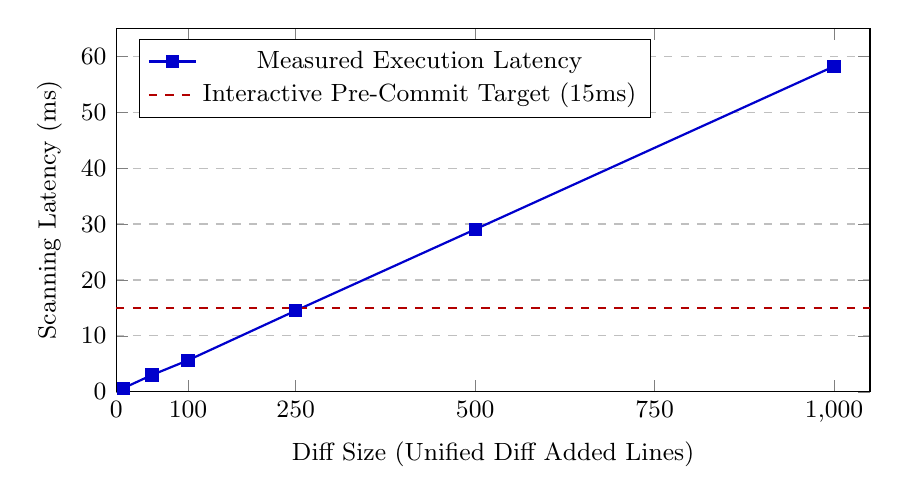
\begin{tikzpicture}
\begin{axis}[
    width=0.92\linewidth,
    height=6.2cm,
    xlabel={Diff Size (Unified Diff Added Lines)},
    ylabel={Scanning Latency (ms)},
    xmin=0, xmax=1050,
    ymin=0, ymax=65,
    xtick={0, 100, 250, 500, 750, 1000},
    ytick={0, 10, 20, 30, 40, 50, 60},
    legend pos=north west,
    ymajorgrids=true,
    grid style=dashed,
    font=\small
]

\addplot[
    color=blue!80!black,
    mark=square*,
    thick
]
coordinates {
    (10, 0.666)
    (50, 3.028)
    (100, 5.646)
    (250, 14.517)
    (500, 29.048)
    (1000, 58.199)
};
\addlegendentry{Measured Execution Latency}

\addplot[
    color=red!70!black,
    dashed,
    thick
]
coordinates {
    (0, 15)
    (1050, 15)
};
\addlegendentry{Interactive Pre-Commit Target (15ms)}

\end{axis}
\end{tikzpicture}

\caption{Measured Scanning Latency as a Function of Unified Diff Size. The measured execution latency scales strictly linearly and remains well below the 15\,ms interactive threshold for commits up to 250 lines.}
\label{fig:latency}
\end{figure}

As depicted in Figure~\ref{fig:latency}, execution latency scales strictly linearly with diff size ($R^2 > 0.999$). For typical pre-commit payloads ($\le 100$ lines), the deterministic extraction engine finishes in $5.65$\,ms, substantially outperforming the 15\,ms interactive threshold. Throughput remains sustained at approximately $17,000$ lines per second across all scales.

\subsection{Ambiguity Scoring and Routing Evaluation (RQ2)}
To evaluate how effectively the mathematical ambiguity metric ($S_{amb}$) separates obvious credentials from ambiguous fixtures, we analyzed five representative candidate patterns traversing diverse contexts.

Table~\ref{tab:routing} details the decomposed terms ($U_{regex}$, $\hat{H}$, $A_{ctx}$), the calculated ambiguity score ($S_{amb}$), and the resulting routing decision.

\begin{table*}[t]
\centering
\caption{Ambiguity Scoring Decomposition and Routing Decisions Across Representative Candidates.}
\label{tab:routing}
\footnotesize
\setlength{\tabcolsep}{3.5pt}
\begin{tabular}{lcccccc}
\toprule
\textbf{Candidate Description} & \textbf{Rule ID} & \textbf{$U_{regex}$} & \textbf{$\hat{H}$} & \textbf{$A_{ctx}$} & \textbf{$S_{amb}$} & \textbf{Routing Decision} \\
\midrule
\texttt{client = boto3.client("s3", aws\_key=...)} & SG-AWS-001 & 0.00 & 0.140 & 0.20 & 0.102 & \textbf{Local Deterministic (0\,ms Network)} \\
\texttt{token = "ghp\_1234567890abcdef..."} & SG-GH-001 & 0.00 & 0.368 & 0.80 & 0.350 & \textbf{Profile A (\texttt{llama-3.1-8b-instant})} \\
\texttt{custom\_auth\_token = "x9aK81mZb..."} & SG-HEUR-001 & 1.00 & 0.260 & 0.20 & 0.538 & \textbf{Profile A (\texttt{llama-3.1-8b-instant})} \\
\texttt{mock\_aws\_key = "AKIAIOSFODNN7E..."} & SG-AWS-001 & 0.00 & 0.140 & 1.00 & 0.342 & \textbf{Profile A (\texttt{llama-3.1-8b-instant})} \\
\texttt{fake\_token = "secret\_test\_mock\_..."} & SG-HEUR-001 & 1.00 & 0.180 & 1.00 & 0.754 & \textbf{Profile B (\texttt{openai/gpt-4o-mini})} \\
\bottomrule
\end{tabular}
\end{table*}

The empirical data demonstrates distinct tier separation:
\begin{itemize}
    \item \textbf{Production Structured Keys:} When a structured AWS key is assigned in production code with explicit sensitive keywords, $U_{regex} = 0.0$ and $A_{ctx} = 0.2$, yielding $S_{amb} = 0.102 < 0.20$. This triggers immediate local resolution with zero network calls and 0\,ms network latency.
    \item \textbf{Test Fixture Escalation:} When an identical AWS key is placed inside a test fixture file, the indicator in the path raises $A_{ctx}$ to $1.00$, escalating $S_{amb}$ from $0.102$ to $0.342$. This routes the candidate to Model Profile A for zero-shot context verification, preventing false alarms on intentional test mocks.
    \item \textbf{Unstructured Generic Tokens:} Heuristic tokens with high entropy in generic contexts receive $U_{regex} = 1.00$, yielding $S_{amb} = 0.538$ (Profile A), while unstructured tokens inside mock test fixtures reach $S_{amb} = 0.754 \ge 0.60$, appropriately routing to high-reasoning Model Profile B.
\end{itemize}

\subsection{Automated Quarantine and Test Verification (RQ3)}
The complete automated test suite comprising 112 test cases across 19 modules was executed via Pytest. The suite verified:
\begin{itemize}
    \item \textbf{Code Refactoring Accuracy:} Verified in \texttt{test\_quarantine.py}. Python files containing string literals were rewritten into \texttt{os.getenv("<VAR>")} assignments without altering indentation or surrounding logic; JavaScript files were successfully converted to \texttt{process.env.<VAR>}.
    \item \textbf{File System Safety:} Quarantined keys were appended to \texttt{.env}, and \texttt{.gitignore} was automatically updated to include \texttt{.env}. When quarantine was cancelled by user abort, source files remained bit-for-bit identical.
    \item \textbf{Overall Test Suite Outcome:} 109 test cases passed and 3 were skipped in $8.64$\,seconds. The 3 skipped tests specifically evaluate POSIX \texttt{chmod 0600} file permissions, which gracefully skip on the Windows host environment without failure.
\end{itemize}
